\documentclass[a4paper,12pt]{article}
\usepackage[russian]{babel}

% Самые необходимые пакеты
\usepackage[T2A]{fontenc}
\usepackage[utf8]{inputenc}
\usepackage[russian]{babel}
\usepackage{geometry}
\usepackage{amsmath}
\usepackage{graphicx}
\usepackage{float} 
\usepackage{xcolor}
\usepackage{listings}
\usepackage{hyperref}
\usepackage{array}
\usepackage{caption}
\usepackage{booktabs}
\usepackage{amssymb}
\usepackage{subcaption}
\usepackage{caption}
\captionsetup[figure]{name=Рисунок}
\usepackage{pgfplots}
\pgfplotsset{compat=1.18}
\usetikzlibrary{arrows.meta}
\usepackage{capt-of}
\usepackage{multirow}
\usepackage[siunitx]{circuitikz}
\usepackage{tikz}
\usetikzlibrary{decorations.markings}
\usepackage{amsthm}
% --- MATLAB code listing style ---
\usepackage{listings}
\usepackage{courier}

\lstdefinestyle{matlab-editor}{
	language=Matlab,
	basicstyle=\footnotesize\ttfamily,      % шрифт Inconsolata
	keywordstyle=\color{blue}\bfseries,     % for, if, while, end
	stringstyle=\color{green!40!black},     % строки
	commentstyle=\color{gray!70}\itshape,   % комментарии %
	morekeywords={...,ode45,atan,vpasolve}, % доп. ключевые слова
	numbers=left,
	numberstyle=\tiny\color{gray},
	numbersep=10pt,
	frame=single,
	rulecolor=\color{gray!40},
	backgroundcolor=\color{gray!4},
	breaklines=true,
	showstringspaces=false,
	tabsize=4,
}
\lstset{style=matlab-editor}


\geometry{left=1.5cm, right=2cm, bottom=2cm, top=2cm}

\usepackage{tocloft}
\renewcommand{\cftsecleader}{\cftdotfill{\cftdotsep}}


\hypersetup{
	hidelinks
}


\begin{document}
	
	% Титульный лист
	\begin{titlepage}
		\centering
		\vspace*{1cm}
		
		% Министерство
		{\small
			Министерство науки и высшего образования Российской Федерации\\
			Федеральное государственное автономное образовательное учреждение\\
			высшего образования\\
			«Национальный исследовательский университет ИТМО»\\
		}
		
		\vspace{2cm}
		
		% Факультет
		{\large
			Факультет систем управления и робототехники\\
		}
		
		\vspace{3cm}
		
		% Основной заголовок
		{\Huge\bfseries
			ОТЧЕТ\\
		}
		\vspace{0.5cm}
		{\LARGE\bfseries
			о практической работе №2\\
		}
		
		\vspace{1cm}
		
		% Дисциплина и тема
		{\Large
			По дисциплине: «Моделирование динамических систем»\\
			\vspace{0.5cm}
			Тема: «Нелинейные системы управления»\\
			\vspace{0.5cm}
			Вариант: 3\\
		}
		
		\vspace{3cm}
		
		\begin{minipage}{0.4\textwidth}
			\raggedright
			{\large
				Студенты:\\
			}
			Охрименко Е. Д.\\
			Комарова О. И.\\
			Чупрова Д. В.\\
			Шишкина М. Н.
		\end{minipage}
		\hfill
		\begin{minipage}{0.4\textwidth}
			\raggedleft
			{\large
				Преподаватель:\\
			}
			Семенов Д. М.\\
		\end{minipage}
		
		\vfill
		
		% Город и год
		{\large
			Санкт-Петербург\\
			2025\\
		}
		
	\end{titlepage}
	
	\newpage
	\tableofcontents
	
	\newpage
	\section{Задание 1.}

	В этом задании мы рассмотрим нелинейную систему:
	
	\[
	\begin{cases}
		\dot{x} = -3x + y \\
		\dot{y} = x - 4y - \arctg2y
	\end{cases}
	\]

	Необходимо:
	\begin{itemize}
		\item Найти положения равновесия системы
		\item Линеаризовать систему около одного из положений равновесия,
		исследовать полученную систему на устойчивость
		\item Доказать устойчивость исходной системы с помощью метода
		функций Ляпунова
		\item Построить графики исходной и линеаризованной систем
	\end{itemize}
	
	\hrule
	\[\]	
	\textbf{Решение: }
	
	Найдем точки равновесия системы:
	
	\[
	\begin{cases}
		-3x + y = 0\\
		x - 4y - \arctg2y = 0
	\end{cases} 
	\quad \Longrightarrow \quad 
	\begin{cases}
		x^* = 0\\
		y^* = 0
	\end{cases} 
	\] 
	
	Теперь линеаризуем исследуемую систему в окрестности точки равновесия \((0, 0)\):

	\[
	J(x) = 
	\begin{bmatrix}
		-3 & 1 \\[6pt]
		1 & -4 - \dfrac{2}{1+4y^2}
	\end{bmatrix} 
	\qquad
	J(0, 0) = 
	\underbrace{\begin{bmatrix}
		-3 & 1 \\[6pt]
		1 & -6
	\end{bmatrix}}_{\text{\large \(A\)}}
	\]

	Далее нужно определить тип положения системы. Найдем собственные значения матрицы \(A\):
	
	\[
	\det\{A - \lambda I\}
	=
	\left|
	\begin{matrix}
		-3 - \lambda & 1 \\[4pt]
		1 & -6 -\lambda 
	\end{matrix}
	\right| = (-3 - \lambda) \cdot (-6 -\lambda ) - 1 \cdot 1 = \lambda^2 +9 \lambda + 17 = 0
	\]
	
	\[\lambda_\text{1,2} = \dfrac{-9 \pm \sqrt{13}}{2}\]
	
	Получаем, что:
	
	\[\lambda_\text{1,2} \in \mathbb{R} \quad \lambda_1 < 0 \quad \lambda_2 < 0\]
	
	Тип системы -- \textbf{устойчивый узел}.\\

	Введём функцию Ляпунова
	\[
	V(x,y) = x^2 + y^2
	\]
	
	Вычислим производную функции $V$ вдоль траекторий системы:
	\[
	\dot V(x,y) = 2x\dot x + 2y\dot y
	= 2x(-3x + y) + 2y\bigl(x - 4y - \arctg(2y)\bigr)
	\]
	
	Раскроем скобки и сгруппируем слагаемые:
	\[
	\dot V(x,y)
	= -6x^2 + 4xy - 8y^2 - 2y\,\arctg(2y)
	\]
	
	Перепишем квадратичную часть в виде суммы квадратов:
	\[
	6x^2 - 4xy + 8y^2
	= 6\left(x - \frac{y}{3}\right)^2 + \frac{22}{3}y^2 > 0
	\quad \forall (x,y)\neq(0,0)
	\]
	
	Тогда
	\[
	\dot V(x,y)
	= -\Bigl(6x^2 - 4xy + 8y^2\Bigr) - 2y\,\arctg(2y)
	= -6\left(x - \frac{y}{3}\right)^2 - \frac{22}{3}y^2 - 2y\,\arctg(2y)
	\]
	
	Заметим, что функция $\arctg(2y)$ монотонно возрастает и нечётна, поэтому
	\[
	y\,\arctg(2y) \ge 0,\quad
	y\,\arctg(2y) = 0 \Longleftrightarrow y = 0
	\]
	
	Следовательно,
	\[
	\dot V(x,y) < 0 \quad \forall (x,y)\in\mathbb{R}^2\setminus\{(0,0)\}
	\]
	
	Из последнего следует, что для введённой функции Ляпунова $V(x,y)$
	и исследуемой системы выполняются условия теоремы об асимптотической
	устойчивости. Таким образом, нулевое решение нелинейной системы
	глобально асимптотически устойчиво.
	
	\qed

	Теперь построим графики исходной и линеаризованной систем:

	\begin{figure}[h!]
		\centering
		
		\begin{minipage}{0.49\textwidth}
			\centering
			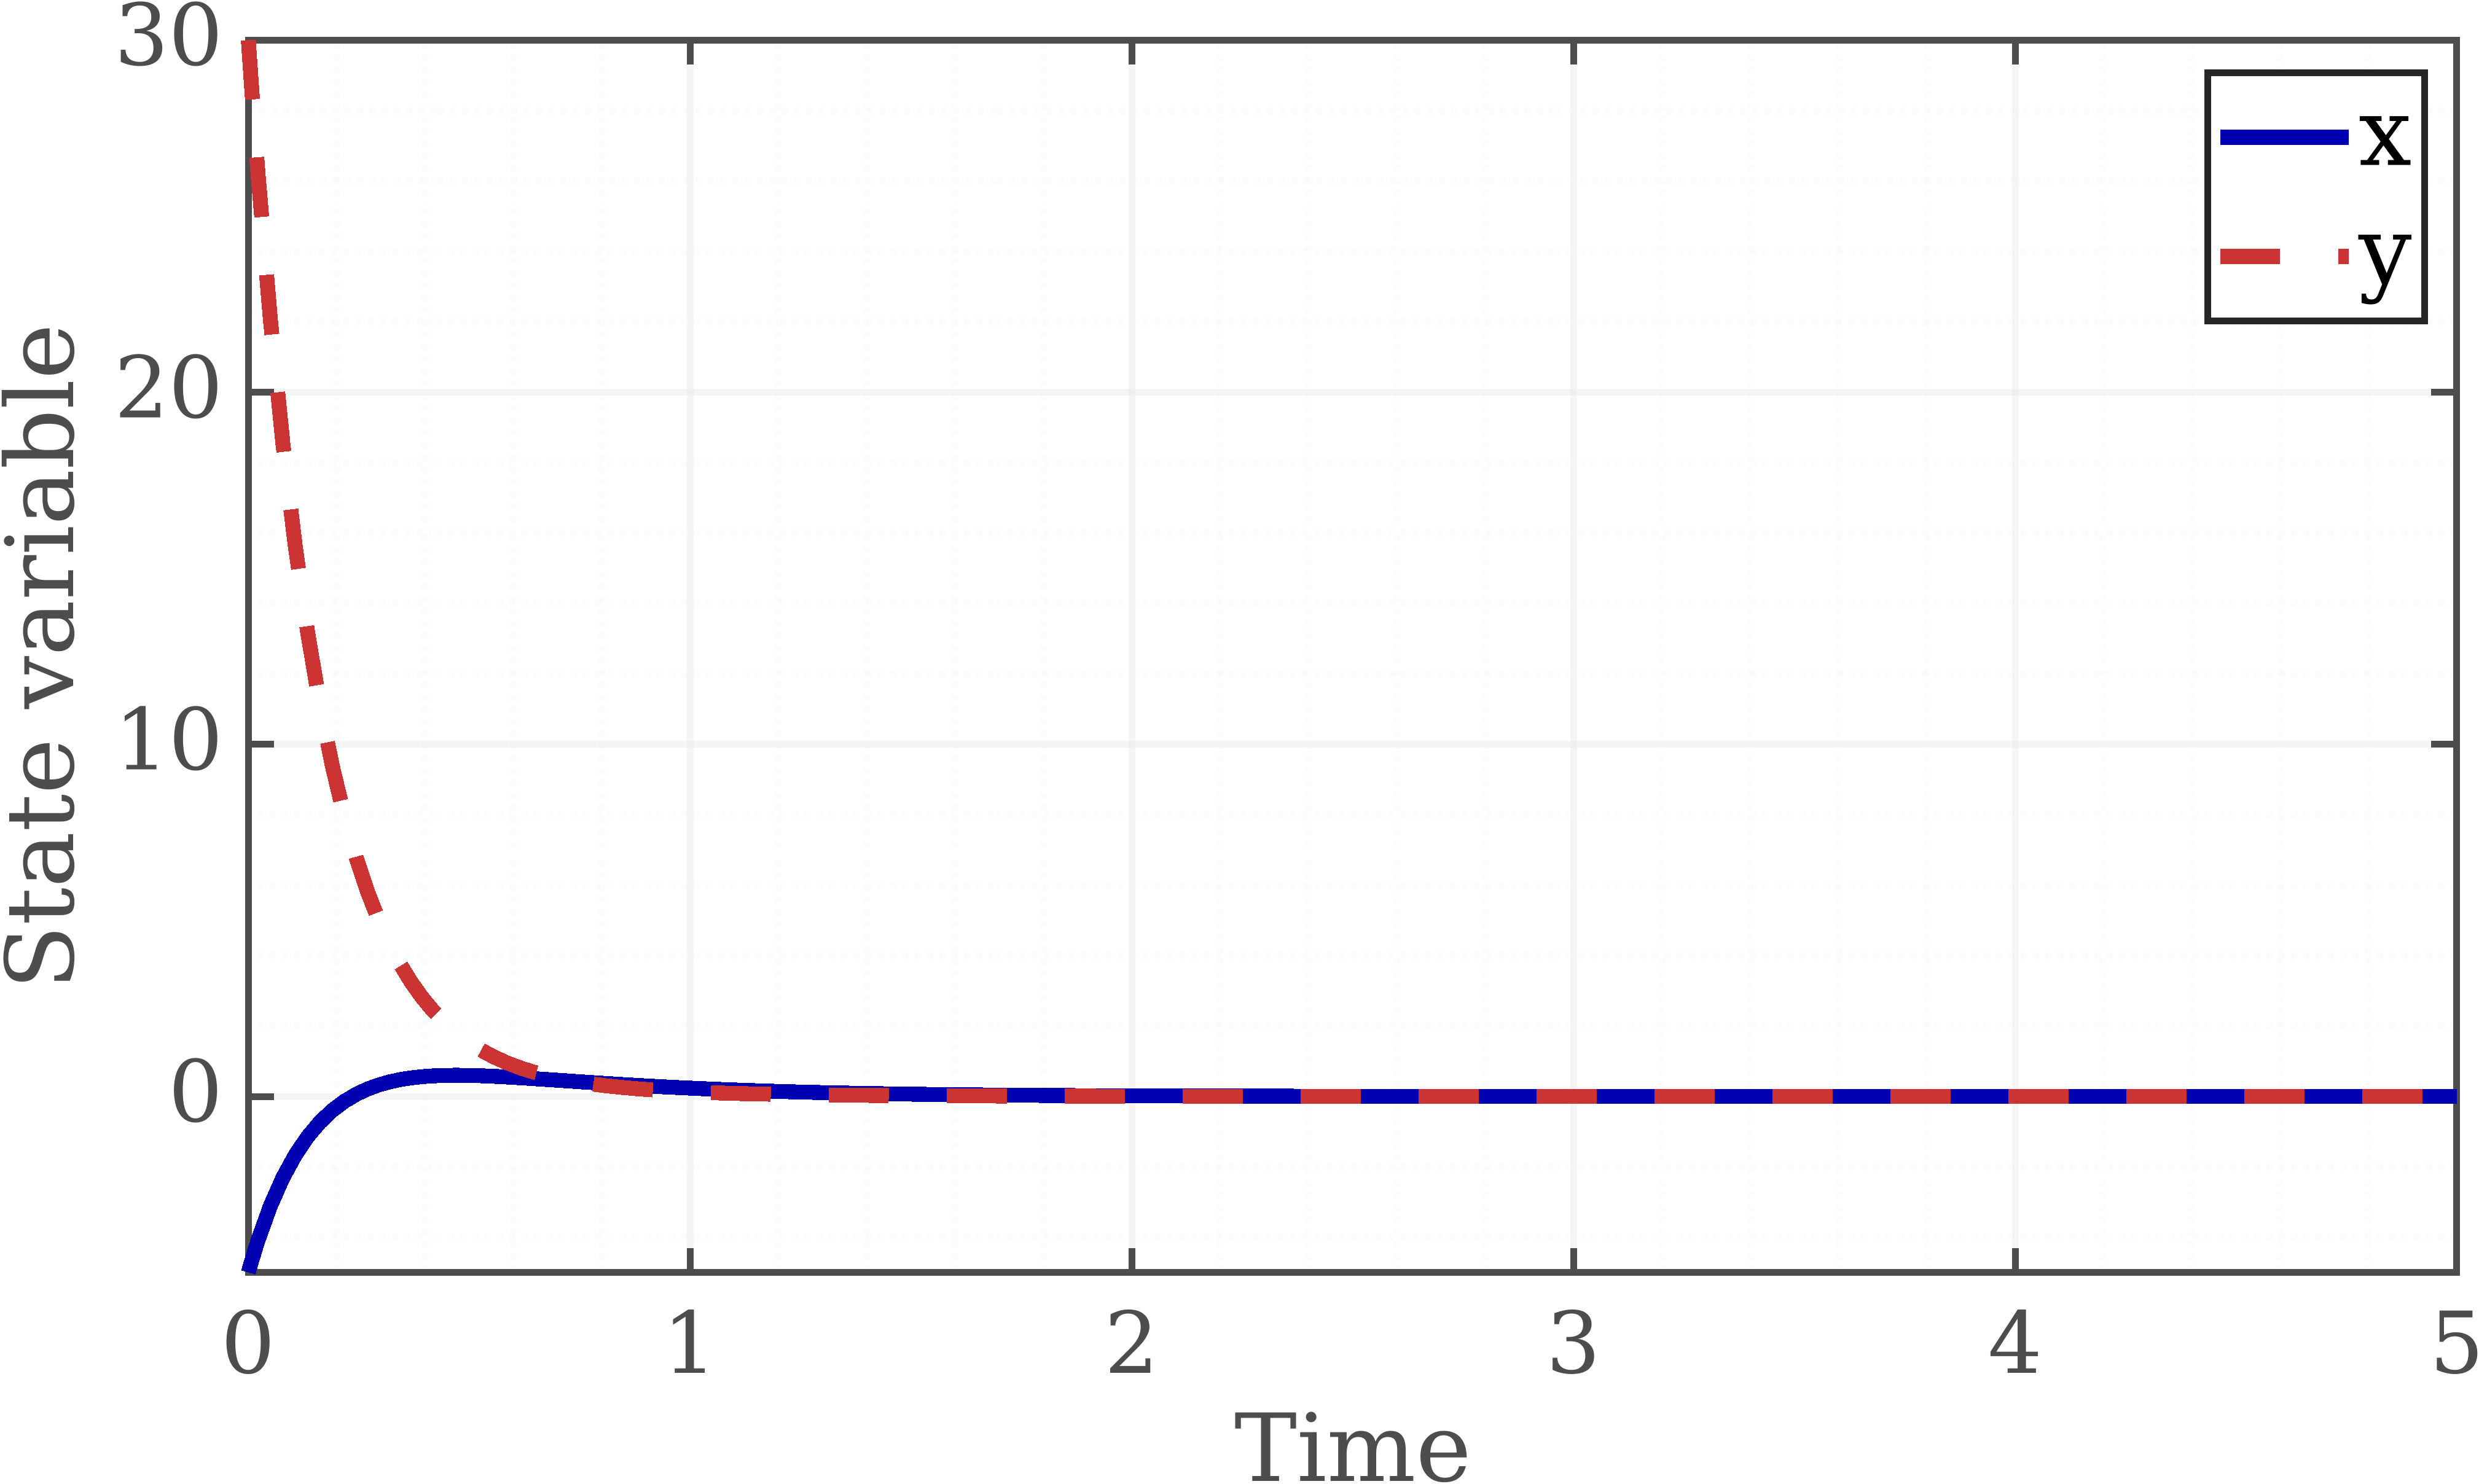
\includegraphics[width=\linewidth]{../images/task1/lin.png}
			(а) Линеаризованная система
		\end{minipage}
		\hfill
		\begin{minipage}{0.49\textwidth}
			\centering
			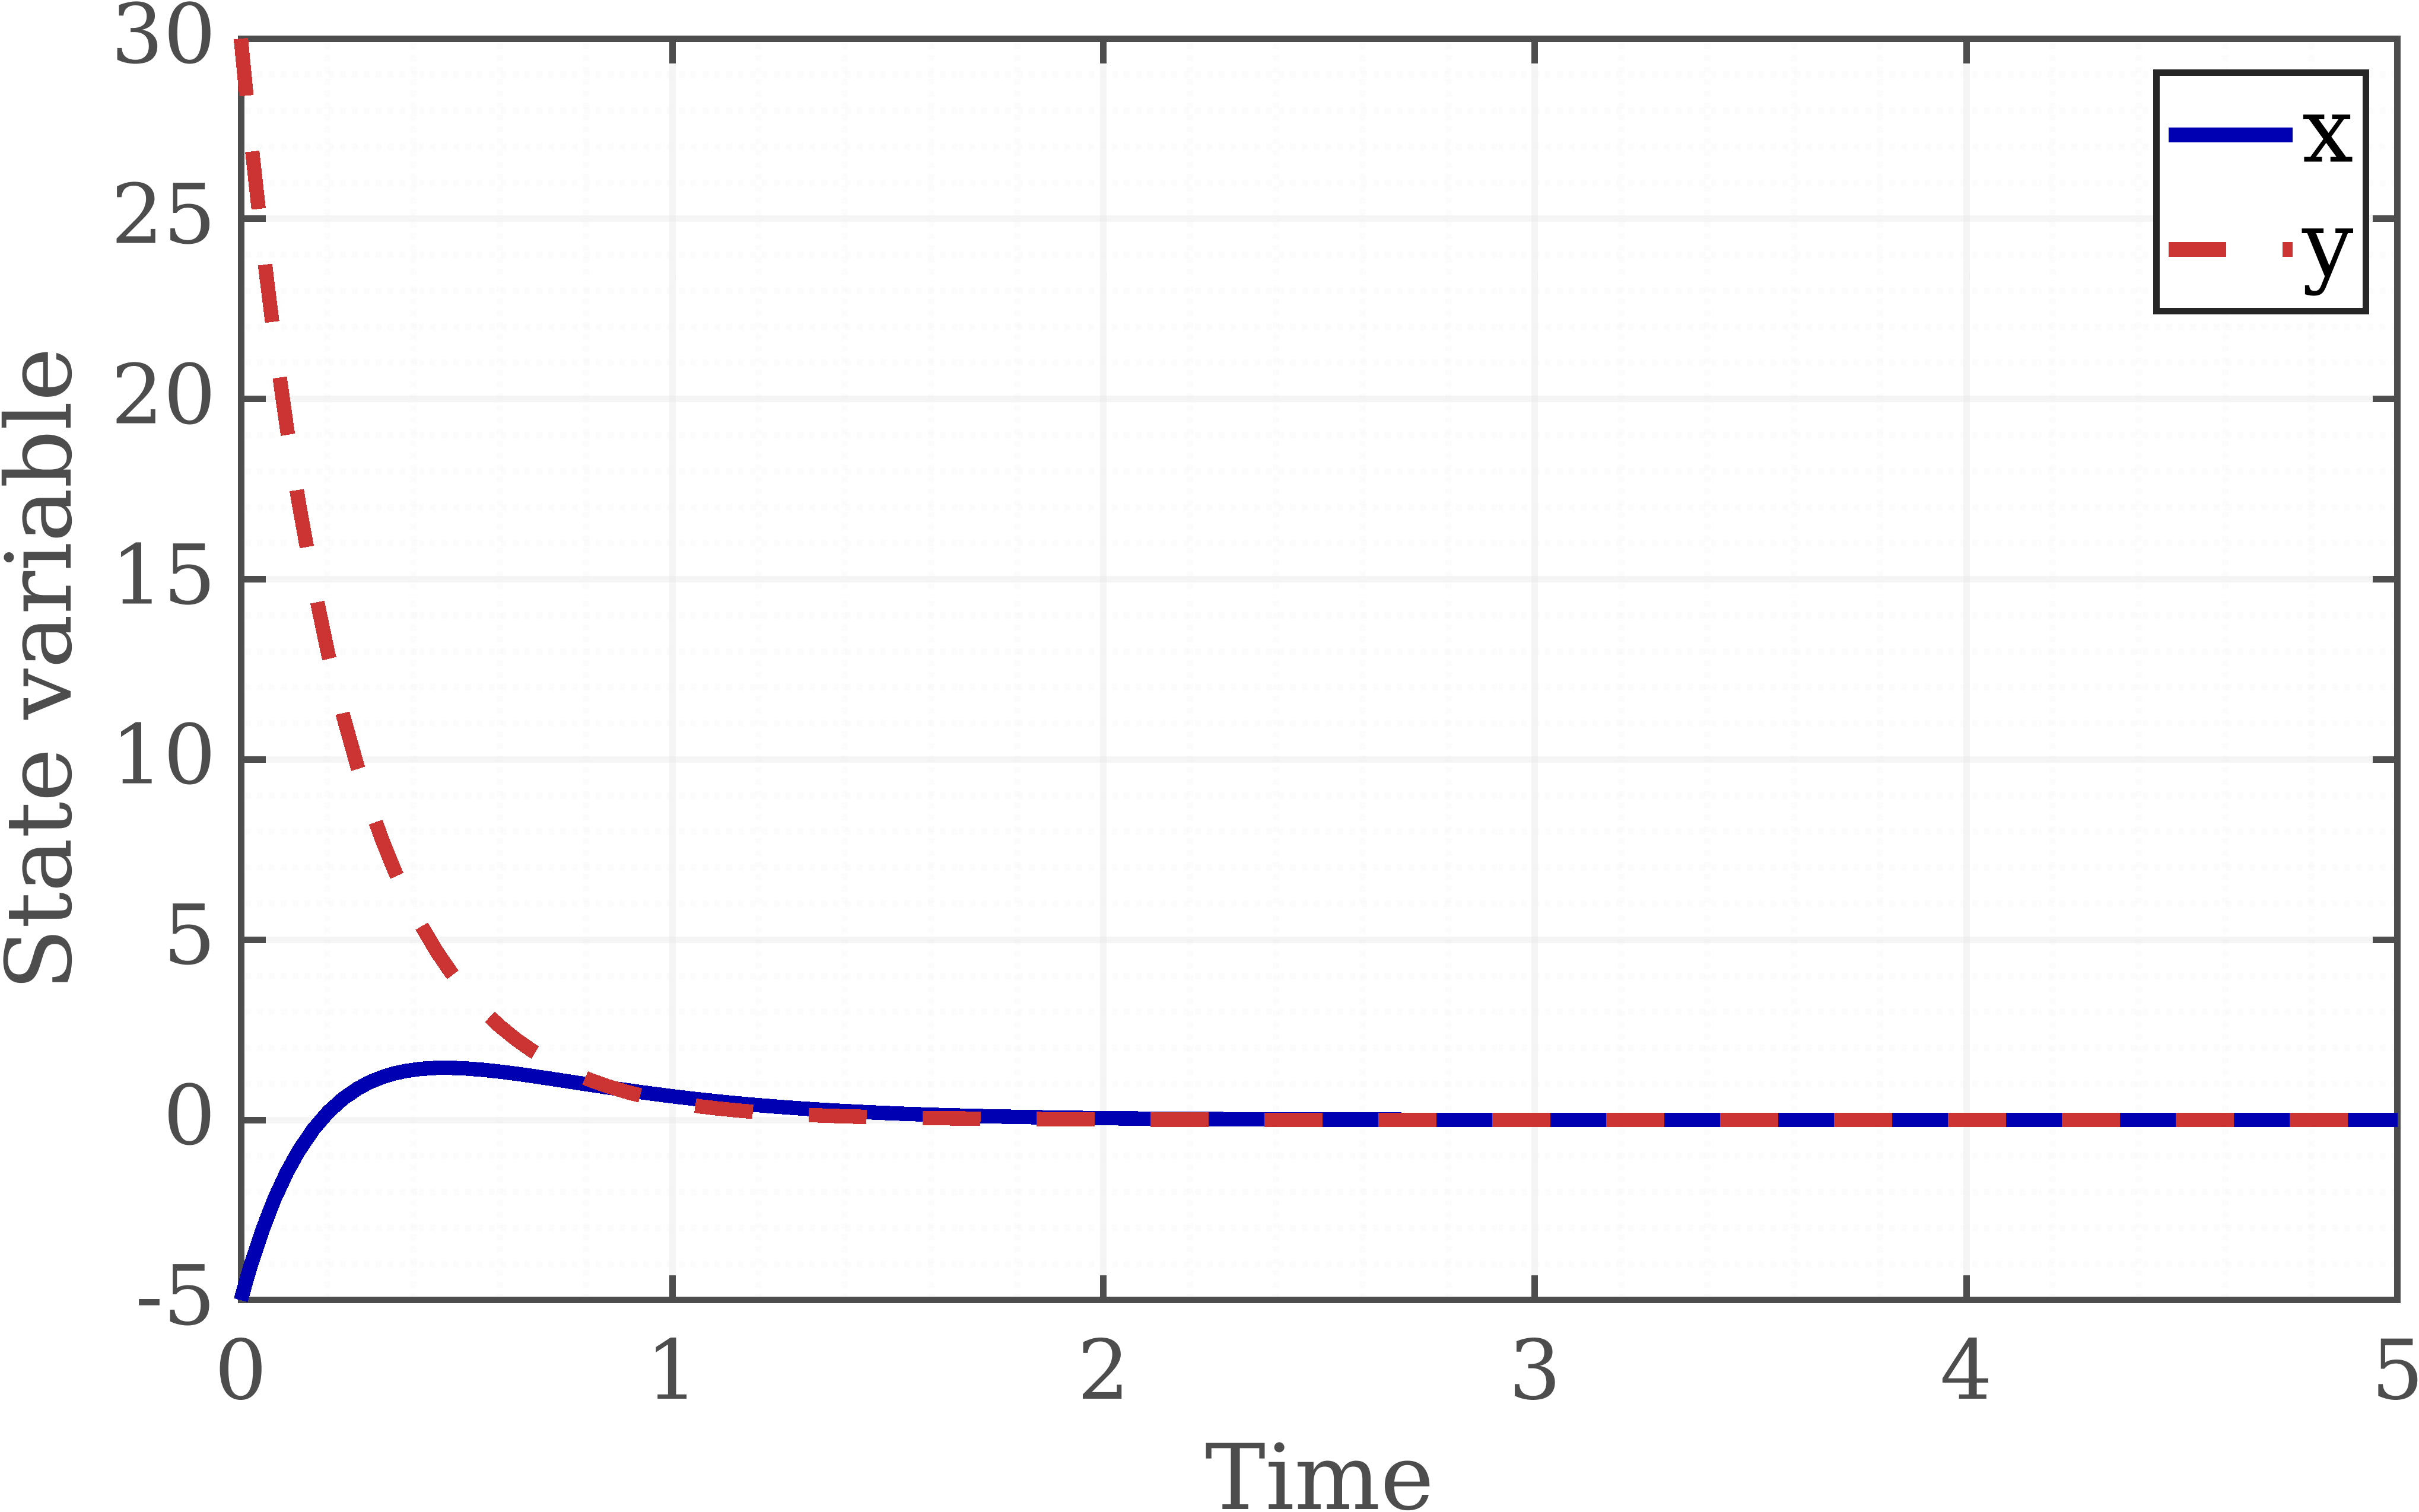
\includegraphics[width=\linewidth]{../images/task1/non-lin.png}
			(б) Исходная система
		\end{minipage}
		
		\caption{Графики динамики линеаризованной и исходной систем}
	\end{figure}
	
	\newpage
	\section{Задание 2.}

	В этом задании рассмотрим нелинейную систему

	\[
	\dot{x} = A x + b\,\xi
	\qquad 
	\sigma = c^{*} x
	\qquad
	\xi = \varphi(\sigma, t)
	\]
	
	где:
	
	\[
	A = 
	\begin{bmatrix}
		-2 & 1 \\
		1 & -2
	\end{bmatrix}
	\qquad
	b =
	\begin{bmatrix}
		1 \\
		0
	\end{bmatrix}
	\qquad
	c =
	\begin{bmatrix}
		1 \\
		0
	\end{bmatrix}
	\qquad
	\xi = \frac{e^{\sigma} - e^{-\sigma}}{e^{\sigma} + e^{-\sigma}}
	\]

	Необходимо: 
	\begin{itemize}
		\item С помощью кругового критерия доказать экспоненциальную устойчивость системы
	\end{itemize}

	\hrule
	\[\]	
	\textbf{Решение: } Пройдемся по всем пунктам кругового критерия.
	

	\begin{enumerate}
		\item Секторное условие.
		
		\[\mu_1 \le	\varphi(\sigma) / \sigma \le \mu_2 \quad \sigma \neq 0 \quad \forall t \in (0, +\infty)\]
		
		В нашем случае представим \(\xi\) как:
		\[\xi = \frac{e^{\sigma} - e^{-\sigma}}{e^{\sigma} + e^{-\sigma}} = \tanh(\sigma)\]
		
		Подставим в условие:
		
		\[\mu_1 \sigma \le \tanh(\sigma) \le \mu_2 \sigma\]
		
		Возьмем производную по \(\sigma\):
		
	    \[\varphi'(\sigma) =  \frac{1}{\cosh(\sigma)}  \in (0, 1]  \quad \forall \sigma\]
	    
	    График функции, проходя через точку \((0, 0)\), имеет наклон не больше 1 и всегда одного знака с \(\sigma\).
	    
	    \begin{figure}[H]
	    	\centering
	    	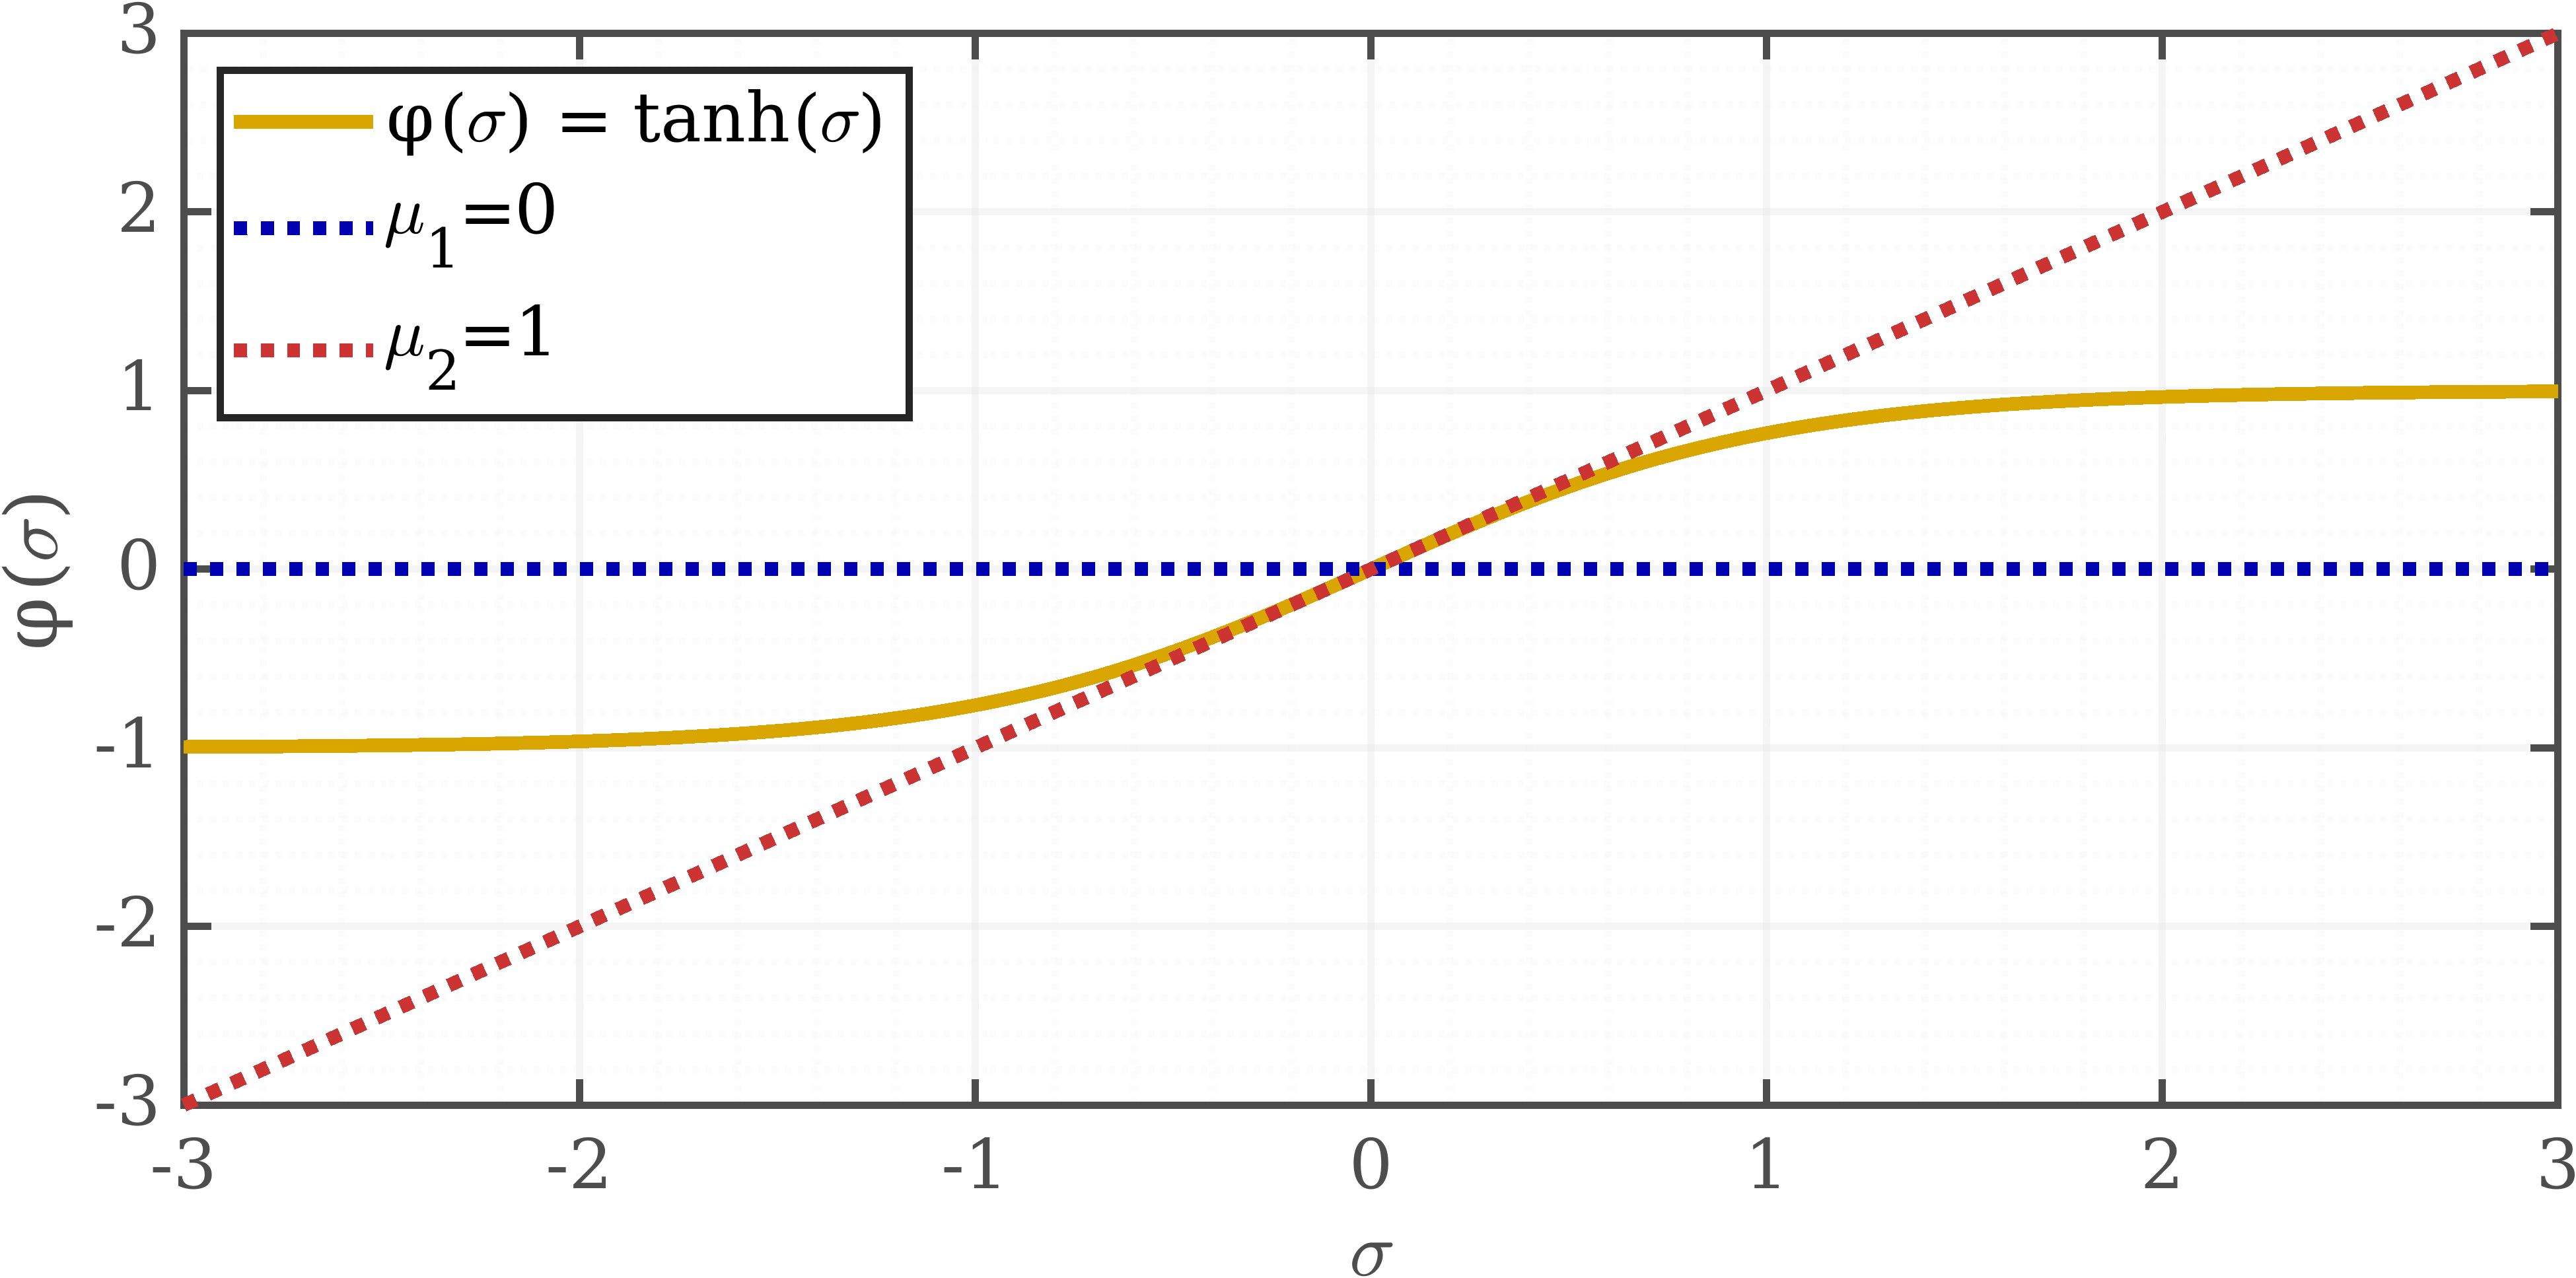
\includegraphics[width=0.8\textwidth]{../images/task2/lines.png}
	    	\caption{Выполнение секторного условия}
	    \end{figure}
	    
	    Отсюда:
	    
	    \[0 < \frac{\tanh(\sigma)}{\sigma} \le 1\]
	    
	    Значит, нелинейность лежит в секторе:
	    
	    \[[\mu_1, \mu_2] = [0, 1]\]
	    
	    Условие выполнено.
	    
	   \item Отсутствие у матрицы \(A\) чисто мнимых собственных значений.
	   
	   Найдем собственные значения матрицы \(A\):
	   
	   	\[
	   \det\{A - \lambda I\}
	   =
	   \left|
	   \begin{matrix}
	   	-2 - \lambda & 1 \\[4pt]
	   	1 & -2 -\lambda 
	   \end{matrix}
	   \right| = (-2 - \lambda) \cdot (-2 -\lambda ) - 1 \cdot 1 = \lambda^2 + 4 \lambda + 3 = 0
	   \]
	   
	   \[\lambda_\text{1,2} = \dfrac{- 4 \pm \sqrt{4}}{2} = 
	   \left[
	   \begin{aligned}
	   	-1\\
	   	-3
	   \end{aligned}
	   \right.
	   \]

	   У матрицы нет чисто мнимых собственных значений, значит это условие выполнено.
	   
	   \item  Асимптотическая устойчивость системы при \(\xi  = \mu_0 \sigma\).
	   
	   Рассмотрим линейную систему:
	   
	   \[\xi = \mu_0 \sigma \quad \dot{x} = (A + \mu_0 b c^T)x \quad b c^T = 
	   \begin{bmatrix}
	   	1 & 0 \\
	   	0 & 0
	   \end{bmatrix}
	   \]
	   
	   Для простоты положим:
	   
	   \[\mu_0 = 0 \in [0, 1]\]
	   
	   Тогда система будет иметь вид:
	   
	   \[\dot{x} = A x\]
	   
	   Так как:
	   
	   \[\lambda_\text{1,2} \in \mathbb{R} \quad \lambda_\text{1,2} < 0\]
	   
	   то матрица \(A\) устойчива, система асимптотически устойчива, условие выполнено.
	   
	   \item Выполнение частотного условия.
	   
	   Найдем передаточную функцию \(W(\lambda)\) с помощью \texttt{MATLAB} (листинг~\ref{lst:Wlambda1}):
	   
	   \[W(\lambda) = c^T(A - \lambda I)^{-1} b  = -\frac{\lambda +2}{\lambda ^2+4\,\lambda +3}\]
	   
	   Теперь положим \(\lambda = i \omega\)  проверим выполнение следующего неравенства:
	   
	   \[\Re\{\left[1 + W(i \omega)\right]^*\} > 0 \quad \omega \in [-\infty, +\infty]\]
	   
	   \[
	   \Re\!\left\{ \left[1 + W(i\omega)\right]^* \right\}
	   =
	   \Re\!\left\{ \left[ 1 - \frac{i \omega + 2}{(i \omega)^2 + 4i \omega + 3} \right]^* \right\}
	   =
	    \Re\!\left\{ \left[\frac{(i \omega)^2 + 3 i \omega + 1}{(i \omega)^2 + 4i \omega + 3} \right]^* \right\}
	   \]
	   
	   Домножим на комплексно-сопряженный знаменатель \( \left((i \omega)^2 - 4i \omega + 3 \right) \). Получим:
	   
	   \[
	   \Re\!\left\{ \left[1 + W(i\omega)\right]^* \right\}
	   =
	    \Re\!\left\{ \left[\frac{((i \omega)^2 + 3 i \omega + 1) \cdot \left((i \omega)^2 - 4i \omega + 3 \right)}{((i \omega)^2 + 4i \omega + 3) \cdot \left((i \omega)^2 - 4i \omega + 3 \right)} \right]^* \right\} =
	   \]
	   
	   \[
	   = \frac{\omega^4 + 8\omega^2 + 3}{\omega^4 + 10\omega^2 + 9} > 0 \quad \forall \omega \in \mathbb{R}
	   \]
	   
		Следовательно, последнее условие выполнено.
		
	\end{enumerate}

	\qed

	\newpage
	\section{Задание 3.}
	
	В этом задании рассмотрим нелинейную систему:
	
	\[
	\dot{x} = A x + b\,\xi
	\qquad 
	\sigma = c^{*} x
	\qquad
	\xi = \varphi(\sigma)
	\]
	
	где:
	
	\[
	A =
	\begin{bmatrix}
		-1 & -3 \\
		-1 & -4
	\end{bmatrix}
	\qquad
	b =
	\begin{bmatrix}
		1 \\
		0
	\end{bmatrix}
	\qquad
	c =
	\begin{bmatrix}
		0 \\
		1
	\end{bmatrix}
	\qquad
	\xi =
	\begin{cases}
		2\sigma & \text{при } |\sigma| < 1\\[6pt]
		2\operatorname{sign}\sigma & \text{при } |\sigma| \ge 1
	\end{cases}
	\]
	
	Необходимо: 
	\begin{itemize}
		\item С помощью критерия Попова доказать асимптотическую устойчивость системы
	\end{itemize}
	
	\hrule
	\[\]	
	\textbf{Решение: } Пройдемся по всем пунктам критерия Попова.
	
	\begin{enumerate}
		\item Секторное условие.
		
		\[
		0 \le \frac{\varphi(\sigma)}{\sigma} \le \mu_0 \le +\infty
		\qquad
		\sigma \ne 0 \quad \forall t \in (0,\infty)
		\]
		
		В нашем случае:
		\[
		\varphi(\sigma) =
		\begin{cases}
			2\sigma & |\sigma| < 1\\[4pt]
			2\,\operatorname{sign}\sigma & |\sigma| \ge 1
		\end{cases}
		\]
		
		Отсюда для $\sigma \ne 0$ имеем:
		\[
		\frac{\varphi(\sigma)}{\sigma} =
		\begin{cases}
			2 & 0<|\sigma| < 1\\[8pt]
			\dfrac{2}{|\sigma|} & |\sigma| \ge 1
		\end{cases}
		\]
		поэтому:
		\[
		0 < \frac{\varphi(\sigma)}{\sigma} \le 2 \qquad \forall\,\sigma\ne 0
		\]
		
		Следовательно, нелинейность принадлежит сектору $[0,2]$, и можно положить $\mu_0 = 2$.
		
		\begin{figure}[H]
			\centering
			
\includegraphics[width=0.8\textwidth]{../images/task3/lines.png}
			\caption{Выполнение секторного условия}
		\end{figure}
		
		\item Устойчивость матрицы \(A\).
		
		Найдем собственные числа матрицы. 
		
		\[
		\det\{A - \lambda I\}
		=
		\left|
		\begin{matrix}
			-1 - \lambda & -3 \\[4pt]
			-1 & -4 -\lambda 
		\end{matrix}
		\right| = (-1 - \lambda) \cdot (-4 -\lambda ) - (-3) \cdot (-1) = \lambda^2 + 5 \lambda + 1 = 0
		\]
		
		\[\lambda_\text{1,2} = \dfrac{- 5 \pm \sqrt{21}}{2} \quad \Longrightarrow \quad \text{Re}(\lambda_{1,2}) < 0\]
		
		Значит матрица \(A\) устойчива.
		
		\item Выполнение частотного условия
		
		Найдем передаточную функцию \(W(\lambda)\) с помощью \texttt{MATLAB} (листинг~\ref{lst:Wlambda2}):
		
		\[
		W(\lambda) = c^T(A - \lambda I)^{-1} b  = \frac{1}{\lambda^2 + 5\lambda + 1}
		\]
		
		Положим \(\lambda = i\omega\). Частотное условие Попова:
		
		\[
		\mu_0^{-1} + \Re\bigl[(1 + i\omega\nu)\,W(i\omega)\bigr] > 0
		\qquad
		\forall\omega \in [0,+\infty]
		\]
		
		Так как нелинейность принадлежит сектору \([0,2]\), то \(\mu_0 = 2\) и
		\(\mu_0^{-1} = \dfrac{1}{2}\). Возьмём \(\nu = 0\). Тогда:
		
		\[
		\frac{1}{2} + \Re W(i\omega) > 0
		\]
		
		Подставим \(W(i\omega)\):
		
		\[
		W(i\omega)
		= \frac{1}{(i\omega)^2 + 5i\omega + 1}
		= \frac{1}{1 - \omega^2 + 5i\omega}
		\]
		
		Домножим числитель и знаменатель на комплексно-сопряжённое выражение
		\((1 - \omega^2 - 5i\omega)\):
		
		\[
		W(i\omega)
		= \frac{1 - \omega^2 - 5i\omega}{(1 - \omega^2)^2 + 25\omega^2}
		\]
		
		Действительная часть:
		
		\[
		\Re W(i\omega)
		= \frac{1 - \omega^2}{(1 - \omega^2)^2 + 25\omega^2}
		\]
		
		Тогда:
		
		\[
		\frac{1}{2} + \Re W(i\omega)
		= 
		\frac{1}{2}
		+
		\frac{1 - \omega^2}{(1 - \omega^2)^2 + 25\omega^2}
		=
		\frac{\omega^4 + 21\omega^2 + 3}
		{2\bigl(\omega^4 + 23\omega^2 + 1\bigr)}  > 0
		\quad \forall\,\omega \in [0,+\infty]
		\]

	\end{enumerate}
	
	Следовательно, критерий Попова выполняется.
	
	\qed
	
	\newpage
	\section{Вывод}
	
	В работе были исследованы три нелинейные системы.  
	
	\begin{itemize}
		\item В первом задании асимптотическая устойчивость подтверждена методом Ляпунова.  
		\item Во втором -- экспоненциальная устойчивость доказана с помощью кругового критерия.  
		\item В третьем -- асимптотическая устойчивость установлена по критерию Попова. 
	\end{itemize}

	Во всех заданиях устойчивость рассмотренных систем подтверждена.
	
	

	\newpage
	\section{Приложение}
	
	\subsection*{Задание 1.}
	
\begin{lstlisting}[caption=Решение системы нелинейных уравнений, language=matlab]
syms x y
eq1 = -3*x + y == 0;
eq2 = x - 4*y - atan(2*y) == 0;

sol = vpasolve([eq1, eq2], [x, y], [0, 0]);
sol.x 
sol.y
\end{lstlisting}

\begin{lstlisting}[caption=Поиск собственных значений матрицы, language=matlab]
A = [-3 1;
	 1 -6];
lambda = eig(A)
\end{lstlisting}

\begin{lstlisting}[caption=Построение графиков систем, language=matlab]
A = [-3 1;
	1 -6];

f = @(t, X)[
	-3*X(1) + X(2);              % x'
	X(1) - 4*X(2) - atan(2*X(2)) % y'
];

lin = @(t, X) A*X;

tspan = [0 5];
X0 = [-5; 30];    

[t1, Xnl] = ode45(f,  tspan, X0);   
[t2, Xlin] = ode45(lin, tspan, X0); 

figure('Position', [100 100 900 500], 'Color','white');
plot(t2, Xlin(:,1), 'Color', [0, 0, 0.7], 'LineStyle', '-', 'LineWidth', 3.5); 
hold on;
plot(t2, Xlin(:,2), 'Color', [0.8 0.2 0.2], 'LineStyle', '--', 'LineWidth', 3.5);

ax = gca; ax.LineWidth = 1.5; ax.FontSize = 20;
ax.XColor = [0.3 0.3 0.3]; ax.YColor = [0.3 0.3 0.3];
ax.GridColor = [0.9 0.9 0.9]; ax.GridAlpha = 0.4;
ax.MinorGridColor = [0.95 0.95 0.95]; ax.MinorGridAlpha = 0.2;
grid on; grid minor; box on; 

xlabel('Time'); ylabel('State variable');
legend('x', 'y', fontsize = 22);
set(findall(gcf, '-property', 'FontName'), 'FontName', 'DejaVu Math TeX Gyre');
exportgraphics(gcf, '../../images/task1/lin.png', 'Resolution', 500);

% % % % % % % % % % % % % % % % % % % % % % % % % % % % % % % % % % % 

figure('Position', [100 100 900 500], 'Color','white');
plot(t1, Xnl(:,1), 'Color', [0, 0, 0.7], 'LineStyle', '-', 'LineWidth', 3.5); 
hold on;
plot(t1, Xnl(:,2), 'Color', [0.8 0.2 0.2], 'LineStyle', '--', 'LineWidth', 3.5);

ax = gca; ax.LineWidth = 1.5; ax.FontSize = 20;
ax.XColor = [0.3 0.3 0.3]; ax.YColor = [0.3 0.3 0.3];
ax.GridColor = [0.9 0.9 0.9]; ax.GridAlpha = 0.4;
ax.MinorGridColor = [0.95 0.95 0.95]; ax.MinorGridAlpha = 0.2;
grid on; grid minor; box on; 

xlabel('Time'); ylabel('State variable');
legend('x', 'y', fontsize = 22);
set(findall(gcf, '-property', 'FontName'), 'FontName', 'DejaVu Math TeX Gyre');
exportgraphics(gcf, '../../images/task1/non-lin.png', 'Resolution', 500);
\end{lstlisting}

	\newpage
	\subsection*{Задание 2.}
	
\begin{lstlisting}[caption=График соблюдения кругового критерия, language=matlab]
sigma = linspace(-3, 3, 1000); phi = tanh(sigma);
mu1 = 0; mu2 = 1;
phi_mu1 = mu1 * sigma; phi_mu2 = mu2 * sigma;

figure('Position', [100 100 900 400], 'Color','white');
plot(sigma, phi, 'LineWidth', 2.5, 'Color', [0.85, 0.65, 0]); hold on;     
plot(sigma, phi_mu1, ':', 'LineWidth', 2.5, 'Color', [0, 0, 0.7]);     
plot(sigma, phi_mu2, ':', 'LineWidth', 2.5, 'Color', [0.8 0.2 0.2]);     

ax = gca; ax.LineWidth = 1.5; ax.FontSize = 15;
ax.XColor = [0.3 0.3 0.3]; ax.YColor = [0.3 0.3 0.3];
ax.GridColor = [0.9 0.9 0.9]; ax.GridAlpha = 0.4;
ax.MinorGridColor = [0.95 0.95 0.95]; ax.MinorGridAlpha = 0.2;
grid on; grid minor; box on; 

xlabel('\sigma'); ylabel('\varphi(\sigma)');
legend({'\varphi(\sigma) = tanh(\sigma)', '\mu_1=0', '\mu_2=1'},'Location','northwest', fontsize = 15);
set(findall(gcf, '-property', 'FontName'), 'FontName', 'DejaVu Math TeX Gyre');
exportgraphics(gcf, '../../images/task2/lines.png', 'Resolution', 500);
\end{lstlisting}

\begin{lstlisting}[caption=Поиск собственных значений матрицы, language=matlab]
A = [-2 1;
	1 -2];
lambda = eig(A)
\end{lstlisting}

\begin{lstlisting}[caption=Поиск передаточной функции, language=matlab, label={lst:Wlambda1}]
syms lambda
A = [-2 1; 1 -2];
b = [1; 0]; c = [1; 0];
W = c.' * inv(A - lambda*eye(2)) * b;
latex(W)
\end{lstlisting}

	\newpage
	\subsection*{Задание 3.}
		
\begin{lstlisting}[caption=График соблюдения кругового критерия, language=matlab]
sigma = linspace(-3, 3, 1000); phi = zeros(size(sigma));
idx = abs(sigma) < 1;
phi(idx)  = 2 * sigma(idx);
phi(~idx) = 2 * sign(sigma(~idx));

mu1 = 0; mu0 = 2;
phi_mu1 = mu1 * sigma;
phi_mu0 = mu0 * sigma;

figure('Position',[100 100 900 400],'Color','white');
plot(sigma, phi, 'LineWidth', 3.0, 'Color', [0.85, 0.65, 0]); hold on;   
plot(sigma, phi_mu1, ':', 'LineWidth', 3.0, 'Color', [0, 0, 0.7]);  
plot(sigma, phi_mu0, ':', 'LineWidth', 3.0, 'Color', [0.8 0.2 0.2]);   

ax = gca; ax.LineWidth = 1.5; ax.FontSize = 15;
ax.XColor = [0.3 0.3 0.3]; ax.YColor = [0.3 0.3 0.3];
ax.GridColor = [0.9 0.9 0.9]; ax.GridAlpha = 0.4;
ax.MinorGridColor = [0.95 0.95 0.95]; ax.MinorGridAlpha = 0.2;
grid on; grid minor; box on; 

xlabel('\sigma'); ylabel('\varphi(\sigma)');
legend({'\varphi(\sigma)', '\mu_1=0 \cdot \sigma', '\mu_2=2 \cdot \sigma'},'Location','northwest', fontsize = 15);
set(findall(gcf, '-property', 'FontName'), 'FontName', 'DejaVu Math TeX Gyre');
exportgraphics(gcf, '../../images/task3/lines.png', 'Resolution', 500);
\end{lstlisting}

\begin{lstlisting}[caption=Поиск собственных значений матрицы, language=matlab]
A = [-1 -3;
-1 -4];
lambda = eig(A)
\end{lstlisting}

\begin{lstlisting}[caption=Поиск передаточной функции, language=matlab, label={lst:Wlambda2}]
A = [-1 -3; -1 -4];
b = [1; 0]; c = [0; 1];
W = c.' * inv(A - lambda*eye(2)) * b;
latex(W)
\end{lstlisting}


\end{document}